\documentclass{amsart}
\usepackage[margin=1in]{geometry}

\usepackage{amssymb}
\usepackage{amscd}


\usepackage{graphics,amsmath,amssymb}
\usepackage{amsthm}
\usepackage{amsfonts}
\usepackage{latexsym}
\usepackage[pdftex]{graphicx}
\usepackage{float}
\usepackage{fancyhdr}

\pagestyle{fancy}
\lhead{Traffic Flow and Safety Analysis Using a Discrete Particle Model}
\chead{}
\rhead{\thepage}
\lfoot{}
\cfoot{}
\rfoot{}

\providecommand{\e}[1]{\ensuremath{\times 10^{#1}}}


\renewcommand{\refname}{}


\title{Traffic Flow and Safety Analysis \\ Using a Discrete Particle Model}
\author{John-Paul Mann, Nathan Minor, Benjamin Squire \\ Central Washington University}


\begin{document}
\DeclareGraphicsExtensions{.pdf,.png,.gif,.jpg}
\bibliographystyle{plain}

\begin{abstract}
Extensive research has been done to model and simulate traffic flow in order to answer valuable questions regarding the implementation of different traffic policies. A major open question is whether or not the stay-right-except-to-pass rule is an efficient traffic policy in terms of traffic flow and safety.  We developed a particle-interaction based model which stems from how cars react and make decisions using locally restricted knowledge, and observed how snap shots of these processes over a large, closed, continuous road affect the dynamics of the overall traffic.  Through our computer simulation, we analyzed the difference between four different traffic policies, or passing rules, which determine how cars react to an impending accident. Specific reactions include passing on the left or right (free passing), passing strictly on the left and then returning to most right lane (single driving), passing on left and then returning to any open lane on the right (single passing), and finally not allowing any passing (no passing) in both low and high density traffic. Our statistical analysis indicated that a free passing rule is both the safest and most efficient passing policy, but further research is needed to determine whether or not other passing policies are more efficient under other, untested, scenarios.
\end{abstract}

\maketitle
\newpage


\tableofcontents
\newpage

\section{\bf{Introduction}}

	
	\subsection{Background}
		All countries implement a set of rules that help regulate traffic and are essential for safe and efficient driving conditions on interstate highways. A common rule, implemented by many countries, states a vehicle must stay in the right-most lane, except to pass a slower vehicle. This means that a vehicle can only pass on the left of another vehicle, returning back to the right-most lane as soon as possible. Compliance is a key factor in the effectiveness of this passing rule. So, the question to be tested is: if people are going to follow this rule will it actually increase efficiency and safety of traffic flow?
	
	\subsection{Approach}
		In order to test the effects of this passing rule on traffic flow and safety, we needed to first establish a model for how our traffic interacts and how the traffic flows as a whole. Essentially, in order to test whether or not a specific passing rule is effective, we cannot rely upon existing data, but instead must create our own data, via computer simulation, in order to model controlled variation in the application of different passing rules. One of the most popular models of highway traffic involves treating the whole system as a pipe filled with fluid and then applying the results of fluid dynamics to measure and analyze the efficiency of the system. Essentially, this a macroscopic model where all control and measuring of the individual interactions is lost.
		
		Another common technique for modeling traffic flow is to analyze individual particle (vehicle) interactions. This approach treats each vehicle as a single particle by analyzing the individual interactions that each vehicle experiences. Our computer simulation follows aspects of both a particle model, which treats each vehicle as an individual particle, while also analyzing the overall dynamics of the roadway. By developing our model to simulate individual interactions between vehicles, we are afford the opportunity to change how a driver responds to each interaction and observe how these interactions affect the overall roadway system. To test the effectiveness of a given passing rule we varied the interaction choices (e.g., passing rule, such as stay-right-except-to-pass or pass whenever and wherever), and  statistically analyzed the hypotheses that the given passing rule was better than another. 

\section{\bfseries{Assumptions and Definitions}}
	\subsection{Definitions}
		\begin{itemize}
  			\item \textit{Highway}: an ideal model of a road with no entries or exit points.
			\item \textit{Vehicle}: an ideal vehicle that all share the same constant length.
			\item \textit{Driving Lane}: a highway lane in which a vehicle is free to travel.
  			\item \textit{Passing Lane}: a highway lane in which a vehicle can only travel in while passing another vehicle.
			\item \textit{Travel Time}: the time it takes for a vehicle to travel a given length of road.
			\item \textit{Traffic Flux}: the rate of cars passing through a given location along the roadway.
			\item \textit{Passing Rule (or Rule)}: a set of distinct choices a vehicle may make during the possible scenarios it might encounter while on the roadway.
			\item \textit{Side-Swipe Accident}: a vehicle collision caused solely by changing lanes.
			\item \textit{Read-End Accident}: a vehicle collision caused solely by a failure to slow down in time.
			\item \textit{Computer Simulation (or Simulation Program)}: the implementation of our model in an Object Oriented Programming Language (OOPL).
			
		\end{itemize}
	
	\subsection{Assumptions}
		General assumptions to this problem turned out to be one of the biggest road blocks that influenced our progress. At every step along the way to choosing a method and developing a model, we had to evaluate and consolidate our previous assumptions with any further assumptions we would need to make in order to maintain a realistic and effective computer simulation. This involved the following major overlaying assumptions:
		\begin{itemize}
			\item	Discrete vehicle speeds and discrete vehicle positions
			\item	Analyze the roadway from the perspective a hot air balloon
			\item 	All vehicles have the same length
			\item 	Internal vehicular performance does not vary
			\item	Lane width, shoulder width, and curvature of road do not significantly affect overall highway dynamics
			\item 	Conservation of Cars: the total number of cars on the roadway remains constant during every simulation
			
			\item  	All roadways are uninterrupted interstate highways
			\item   Crashes are not simulated and, thus, have no effect on dynamics of highway
			\item 	Severity of all accidents considered equivalent			
		\end{itemize}
		 
		In order to improve the tractability of our model, we had to make the assumption that the speeds and positions of vehicles are both discrete quantities. There are two reasons why this is a reasonable assumption to make: simulates the realistic snapshot data of real interstate highways, and allows for the ability to scale our model. The discrete speeds and positions can be interpreted as snapshots of the highway at constant time intervals, such as one second. This says that, within our computer simulation, each iteration is simply a snapshot of the highway at a particular time. Thus, by scaling time and position discretely, our model simulates what it is like to look at a sequence of photos which make up an 8 minute time lapse of traffic on an interstate highway. As for speed, once we assume discrete vehicle positions, it only makes sense to have the vehicle speeds defined in discrete quantities as well. As a side note, there is a lot of research on how very small deviations in speed can grow traffic jams quickly in places that would not be expected \cite{kurttraffic}. Since we only use discrete quantities for our vehicle speeds and positions, these ''phantom'' traffic jams do not appear in our model.
	
		Hot Air Balloon Perspective is a perspective assumption based on a view of the whole section of the highway at a single time instead of an internal perspective where we are measuring from inside the system. This plays into both the programming of the model as well as the macroscopic measuring of the system. 
		
		A constant vehicle length can be assumed due to only slight variations in actual vehicle length. Also, since there are discrete position intervals, a vehicle can only be integer lengths of these discrete position intervals. As for modeling longer vehicles, the model allows for two constant length vehicles to be connected in line at a specific speed.

		Internal vehicular performance is in reference to the assumption that all cars break, accelerate, and function at equivalent performance levels. This assumption addresses a more subtle aspect of similar that would only increase the complexity of our model without increasing the effectiveness of our model to test different passing rules. Also, by the assumption that vehicles travel at discrete speeds, internal vehicular performance should not vary on a vehicle-to-vehicle basis. 

		Lane width, shoulder width, and curvature of the road are assumed to have no effect on testing the effects of different passing rules. In general, lane widths on a highway have such small variations that any difference is assumed to have nominal effect on the ability to switch lanes. Also, smaller lanes allow faster lane changes but decrease traveling safety so the assumption is these small variations do not affect safety. Same principles also apply to highway shoulders and median variations. No oncoming traffic is assumed so the median consideration is unnecessary at this stage of research. The median is assumed to be so wide that the oncoming traffic has no effect on the decision making ability of vehicles on the roadway. In the analysis of real traffic data, shoulder width is seen to have an effect on a driver's safety perception, but we are assuming that this has no significant influence on the effects of a particular passing rule \cite{elvik2009handbook}.
		 
		 Conservation of cars is a combination of factors: no vehicles enter mid-way through the highway and the traffic density of the entire roadway is constant. This correlates to no exit or entry ramps on this stretch of the highway our computer simulation models, and as a vehicle exits the highway another vehicle enters the highway. This assumption is mostly intended to simplify the implementation of our model in an object-oriented programming language. However, as the length of the roadway is increased, the inaccuracies (that might be caused by assuming a conservation of cars) are minimized because it will take longer for a vehicle to pass through the roadway more than once. To further justify this assumption, reference can be made to a large percentage of traffic models that also make this assumption \cite{seiboldconstructing}. 
		 
		 In our definition of a highway the assumption was already made that there are no exits or entry ramps midway through the highway. Furthermore, we want to exclude any slowing or stopping due to traffic lights, intersections, accidents or further impairments since these should not have an effect on the testing of different passing rules. Our model allows for these traffic impairments to be incorporated, with minimal changes to the source code, but at this stage of our research it would not improve the accuracy of our model enough to warrant these extra complexities. 

		In our model we calculate the amount of accidents that are likely to result on a highway, while simultaneously assuming that a crash will not stop or slow down traffic. A major reason for making this assumption is to simplify the implementation of our model into an object-oriented programming language. However, more importantly, this assumption is justified because we want to test crashes caused only by different passing rules. If we allowed accidents to slow down traffic, the results of our computer simulation would not just show the effects of different passing rule, but also the additional effects caused vehicle accidents.

	Although there are different probabilities associated with side-swipe accidents versus rear-end accidents, no severity of accident is incorporated into our model. This implies that the safety of the roadway is not associated with how bad accidents on the roadway actually are. With further research we can factor in the severity of each accident, but that would added unnecessary complexity to our model.
		
\section{\bfseries{Development of Method}}
	\subsection{Method Rational}
	In our approach to testing different passing rules, we wanted to develop an effective model for traffic interactions that could generate data for a set of passing rules on a given stretch of road. This would allow for greater variation of parameters and assumptions, instead of relying on data collected for a specific highway with (possibly) different assumptions and passing rules. Furthermore, if we develop a model that has very specific parameter variation capabilities, then the data for for different passing rules under different roadway scenarios would be easier to collect, analyze, and interpret. 
	
	Initially there were three general model ideas that we considered in order to create a model that allows for the variation of different parameters. The first model we considered was a single particle model that would effectively model each individual interaction of a vehicle trying to pass another vehicle. The other extreme was to consider the macroscopic idea of modeling the highway as a whole, and to use differential equations to model the rate of flow for traffic. The third model we considered developing was some combination of the particle model and fluid dynamics model \cite{burghout2005}.
		
		\subsubsection{\it Fluid Dynamics}
		In the realm of macroscopic traffic modeling, fluid dynamics is a popular and common technique. The idea behind this technique is that cars in heavy traffic interact similar to particles, either gas or liquid, in a confined tube. The main difference between gas and liquid is compressibility, or the ability to change density of the fluid. A gas model is said to be compressible, allowing changes in  fluid density. While a liquid model is said to be incompressible, allowing no change in fluid density \cite{stone2007introduction}. The majority of fluid dynamical models that we considered implemented incompressible fluids on both a macroscopic and microscopic model. Originally, we tried to vary viscosity within the fluid and vary the shape of the tube the fluid traveled through. By varying viscosity then the high viscosity pockets of fluid would represent pockets of slower traffic, while low viscosity fluid would represent pockets of faster traffic. The other technique replaced pockets of slower traffic with unmovable obstructions as part of the pipe wall or shape. 
		
		\subsubsection{\it Discrete Particle Model}
		
	The other extreme that we tried to pursue for our model involved a discrete particle model that simulated individual interactions. In this model we were hoping to create a program that modeled the specific characteristics of interactions under a particular passing rule. By evaluating the different parameters that constitute every passing interaction, the resulting data would shed light on the efficiency of the stay-right-except-to-pass rule. Additionally, this model would provide the ability to measure the safety of passing on the right versus passing on the left, the amount of time required for each passing interaction, the effect passing has on the immediate properties of each vehicle, etc. 
	
	However, within this model we start to lose sight of the overall highway. By only considering a few interactions at a time it is almost impossible to see traffic jams develop, changes in highway flow, or density of the highway. If we are not able to test these factors then it would be hard to say whether different passing rules had any effect on the efficiency of the highway as a whole.
		
		\subsubsection{Mixed Model}
		
	Eventually, an obvious conclusion was to find an effective median between the macroscopic fluid dynamics and the discrete particle models. We decided to start with the discrete particle model and slowly generalize it into a macroscopic situation by considering the overall system dynamics. By utilizing the particle model we had an effective way to vary the actual interaction between every single vehicle. This gave us complete control over what actually happens when a vehicle tries to pass another vehicle. 
	
	The very first model that we fully developed was a very basic computer simulation that produced data we could illustrate on graph paper. This original program only had a road length of 100 units (or tiles), with discrete vehicle positions and speeds. As we drew out the positions we began to discover not only the bugs within the computer simulation, but also in the short length of road and vehicular speed classes of 1,2, or 3 tiles per iteration. We were also able to identify which data points from the computer simulation we wanted to track in order to statistically analyze a set of passing rules against another set of passing rules.

	\subsection{Discrepancies of Fluid Dynamics}
	Immediately, a major problem with the fluid dynamics model was creating a solution to implement different passing rules into a fluid's attributes. Since we were unsuccessful in finding an already existing model that allowed for this variation in passing rules, the technique we pursued was implementing a system containing a fluid with non-unified viscosity. 
	
	One problem that appeared with using results from fluid dynamics was the models ability to accurately simulate traffic dynamics as density decreases \cite{stone2007introduction}. This is because, as traffic density decreases on a roadway there appear large gaps in the traffic that would not be present in either a liquid or a gas, even if we allowed the fluid to be compressible. One variation in parameters that we considered important for testing the effects of a given passing rule was the change between low and high density traffic. Some models attempted to adjust for density by varying viscosity of the fluid as we had hoped. In these cases though the differential equation analysis became more and more complicated as the viscosity varied. Since we felt our model required large variations in viscosity in small intervals we were led to the conclusion that all these assumptions generalized the fluid into too macroscopic of a model to properly simulate the individual interactions between vehicles effectively. 

	We further investigated other theories in the fluid dynamics model, but found that none these models allow the use of a particle specific rule that would quantify a passing rule. Therefore, we decided not to pursue a model based solely in fluid dynamics \cite{piccolireview}.
	

\section{\bfseries{Road Rules}}
	The stay-right-except-to-pass rule becomes more difficult to describe as the highway becomes three or more lanes wide. Essentially, there are two different rules that this stay-right-except-to-pass rule breaks down into when three or more lanes are present on an interstate highway. There is the rule that all drivers must remain as far right as possible (except to pass another vehicle), and the rule that there is a single left-most passing lane and drivers can travel within the remaining other lanes freely. In order to test all variations in passing tendencies, we developed the following passing rules:
		\begin{itemize}
			\item No Passing Allowed,
			\item Free Passing,
			\item Single Passing Lane, and
			\item Single Driving Lane.
		\end{itemize}

	\subsection{No Passing Allowed}
	The No Passing Allowed Rule states that all lanes on the highway are driving lanes and that there is no passing involved in the system. Under this rule a vehicle will remain in the lane that it started in for the entirety of its travel. An obvious result of this passing rule is that there will be large chains of cars all going the same speed. When there are two or more lanes on a stretch of highway this passing rule has no practical application, which supports why we are developing it as a control variable. 
	
	However, there are applications to this rule when the highway only has one lane traffic. For example, in a construction zone or on a highway where there is only one lane traffic in each direction and the oncoming traffic is too heavy to pass. In these cases, this No Passing Allowed Rule can provide effective insight into the clustering of different speed pockets. Our research is not concerned with speed pockets, so we will simply think of this No Passing Allowed Rule as a base case that represents an extreme in the spectrum of passing rules. 
	\subsection{Free Passing}
	The Free Passing Rule states that the vehicle will continue in its current lane until it approaches another vehicle in its lane. When a slower vehicle is in front of a faster vehicle, the faster vehicle will attempt to change lanes. The faster vehicle will first try to pass the slower vehicle on the left, but if there is no lane open to the left then the vehicle will attempt to pass to the right. If passing is not possible in either direction, then the faster vehicle will decrease its speed until its speed matches the slower vehicle's speed.

	Therefore there are two important differences in this passing rule than in the other passing rules: the direction of passing and the action after lane changing. Under this rule vehicles can pass going either to the left or to the right. Also, once a vehicle does change lanes it will remain in that lane until it is forced to pass again. 

	Furthermore, this passing rule provides us with a model that shows the absence of any passing laws. In a practical application, most cars do not operate by this Free Passing Rule, but there are individuals who interact with other vehicles in this manner. The real importance of this passing rule is that it provides a control case on the other extreme of the passing rule spectrum, opposite that of the No Passing Allowed Rule. The Free Passing Rule says that there is an absence of any rules regarding passing and, thus, may provide an argument that passing rules need to be implemented to improve efficiency and safety. 
	
	\subsection{Single Passing Lane}
	The Single Passing Rule states that there is only a single passing lane on a multilane highway, and the remaining lanes are designated as driving lanes. A Single Passing Rule and a Single Driving Rule are equivalent on a one or two lane highway. This rule was created in order to account for more driving lanes than the farthest right lane for highways of more than two lanes. Therefore any lane that is not the farthest right or the farthest left lanes allows both driving and passing within it. 
	
	This rule can be assumed to closely mirror how heavy traffic flow works on a busy multilane highway. Drivers tend to leave the left-most lane empty for passing or carpooling, while driving in all other lanes of traffic without the need to gravitate to the right most lane. We have not included a carpool lane because we are not making any assumptions about the number of passengers in any given vehicle.
	
	\subsection{Single Driving Lane}
	The Single Driving Rule states that the farthest right lane is a driving lane and all other lanes on the highway are strictly passing lanes. A Single Driving Rule and a Single Passing Rule are equivalent on a one or two lane highway. 

	This rule tests the stay right except to pass law most efficiently. By forcing drivers to only travel in the right lane except while passing the system takes into effect that a vehicle has to return to the same lane they were previously traveling in before overtaking another vehicle. Therefore this rule must be tested against the efficiency and safety of all the other rules in order to actually test the stay right except to pass law. 

\section{\bfseries{Modeling}}

\textit{\textbf{Model Specific Definitions}}

\begin{itemize}
	\item \textit{Initial Speed}: speed of an individual vehicle at the start of a computer simulation
	\item \textit{Current Speed}: speed of an individual vehicle for the current iteration of a computer simulation
	\item \textit{Iteration Average Speed}: the average current speed of all vehicles on the highway for a given iteration of a computer simulation
	\item \textit{Highway Density}: amount of cars per unit length over the whole highway; constant in current model
	\item \textit{Traffic Flux}: the average speed multiplied by the highway's density
	\item \textit{Road Type}: initial conditions of a highway based on density (high or low) and lane count (2-5)
	\item \textit{Simulation}: a collection of iterations over a given set of distinct road types
	\item \textit{Average Simulation Speed}: the average speed for a certain road type during a particular simulation
	\item \textit{Simulation Iteration}: distinct interval of time represented by each iteration; our model assumes a one second duration per iteration 
	\item \textit{Simulation Parameters}: the computer program's initial variables: number of simulations to run, which passing rule to implement, number of roads (determines the number of different road types being tested), length of road, and iterations per simulation
	\item \textit{Summary Data}: the type of data output by the computer program: lane count, traffic density, average speed, total slow downs, total lane changes, total decisions
	\item \textit{Road Summary Data}: summary data for an individual road type after each iteration
	\item \textit{Simulation Summary Data}: summary data for each simulation
	\item \textit{Safety Rating}: scaled probability of an accident occurring during a simulation
	
\end{itemize}
	
\textit{\textbf{Model Specific Assumptions}}

	\begin{itemize}
	\item Normal Distribution of Initial Speed
	\item Speed Increases to Initial Speed When Possible
	\item Mirrored Traffic Assumption	
	\item All overlying assumptions stated previously.
	
\end{itemize}

\textit{Justifications}\\

	Initial speed of the vehicles on the highway is determined by a normal distribution. We are making this assumption to maximize the accuracy of our model. Speeds in the current scaling of the system are taken to range from 54 MPH to 90 MPH. This sets the average speed of the highway at 70 MPH which is a common speed limit for interstate highways in the United States. By normally distributing initial speeds the break downs are:

\begin{figure}[h]
\centering
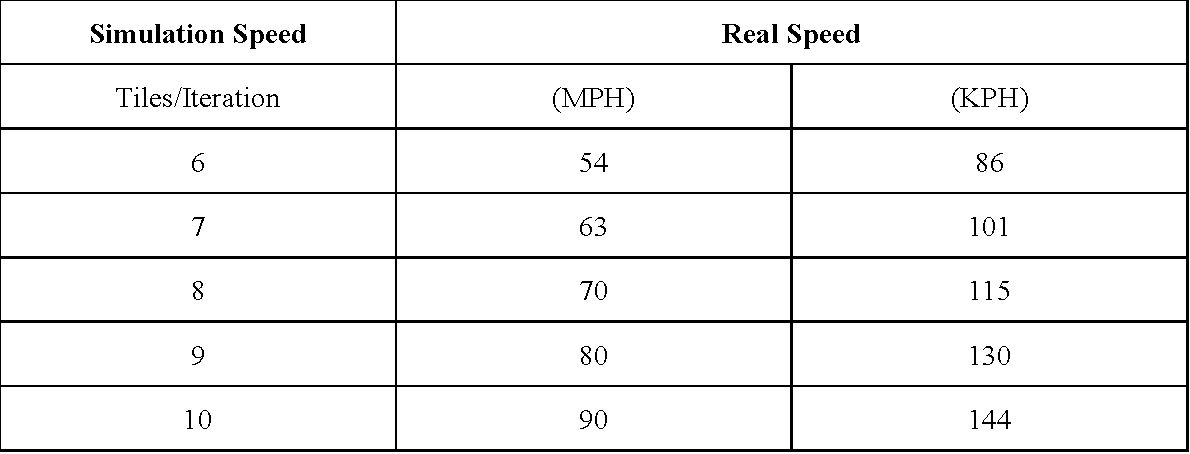
\includegraphics[scale=0.5]{MCM-SimulationSpeedTable.pdf}
\caption{Comparison scale of speed within model to the representation in real speeds.}
\label{MCM-SimulationSpeedTable}
\end{figure}

	Inside the simulation, vehicles are often slowing down since no crashes are allowed in the system. Therefore we assume that every vehicle wants to accelerate back to it's initial speed as soon as it possibly can. This is an important assumption to make in terms of the accuracy of our model because on real highways individual drivers tend to drive at a steady average speed when their path is not impeded. 
	
	Furthermore, we are making the assumption that traffic which drives on the left side of the road, such as in the United Kingdom, is simply a mirror image of traffic that drives on the right side of the road, such as in the United States. Thus, staying right except to pass on the left is the same as staying left except to pass on the right. Additionally, switching lanes to the left is assumed to be the same as switching lanes on the right.
	
	\subsection{Implementation of Model}
	
		\subsubsection{Why Java and XML?}
			
			We chose to implement our traffic model using Java for two main reasons. We wanted to use a language that allowed us to encapsulate our model in a class structure. Thus, the high-level language and object-orientated structure of Java was our foremost reason for implementing our model in Java. Additionally, we chose Java over other object-orientated, high-level languages because our familiarity with programming in Java out-weighed our desire to learn the ins-and-outs of an unfamiliar high-level language.
			
			As for the persistence of our simulation summary data, we chose to use the data persistence functionality of Extensible Markup Language (XML) because of the ability within Java to easily convert data encapsulated in our class structure to XML data encapsulated in Java packages that handle Java-to-XML interactions. Furthermore, XML is a standard data persistence language that easily imports into many different types of data analysis software, such as Microsoft Excel. 
			
		\subsubsection{Encapsulation of Model with Object Orientation}
		
		As mentioned above, we wanted to make use of object orientation to encapsulate our model into a class structure. Due to time constraints we minimized the class structure of our simulation program to include only the functionality and data encapsulation necessary to fully implement our model. Below is a breakdown of the functionality and data encapsulation for each class in our program.
		
		\begin{enumerate}
			\item{\textbf{\texttt{Car}}
				This class encapsulates the initial speed of a vehicle, determined by our normal distribution of vehicle speeds, the current speed of a vehicle, changed by our logic tree (see Figure ~\ref{MCM-LogicalFlowChart}.), and the passing state of a vehicle, either true of false. 
			}
			\item{\textbf{\texttt{DataPersistence}}
				This class encapsulates the functionality for persisting the simulation summary data into an XML file. This class handles the conversion of the encapsulation of the simulation summary data to data in an XML file using \texttt{java.io.*}, \texttt{java.xml.*}, \texttt{org.w3c.dom.*} packages.
			}
			\item{\textbf{\texttt{Main}}
				This class is the entry point for the flow of execution of our simulation program. The interface for prompting a user for the simulation parameters and looping structure for running multiple simulations with the same parameters are encapsulated in this entry-point class.
			}
			\item{\textbf{\texttt{Map}}
				This class encapsulates a collection of roads that a simulation tests. Each road in the \texttt{Map} represents a different road type that the simulation tests with a specific rule.
			}
			\item{\textbf{\texttt{Position}}
				This class encapsulates a position on a road by the lane and slot (length-wise position) values.
			}
			\item{\textbf{\texttt{Road}}
				This class encapsulates the properties of a road in our simulation, based on our assumptions. These properties include the number of lanes, the length of the road, the traffic on the road (i.e., a collection of cars), and counts of the number of decisions, lane changes and slow downs that occurred during an iteration of our simulation program. Since our model assumes a hot air perspective, the array used to store the cars on a road has the dimensions of road, as seen from a hot air balloon, and the position of each vehicle (in terms of lane and slot) are the indices of the vehicle object in the array.
			}
			\item{\textbf{\texttt{Rules}}
				This enumerator class encapsulates a designation of the rule used to navigate our logic tree (see Figure ~\ref{MCM-LogicalFlowChart}.) during a simulation. The values stored in this enumerator class are \texttt{FREE PASSING, SINGLE PASSING, SINGLE DRIVING, NO PASSING}.
			}
			\item{\textbf{\texttt{Simulation}}
				This class encapsulates a collection of different road types that different numbers of lanes and different traffic densities to test how these parameters, in conjunction with a rule, affect the flow of traffic on a road type.
			}
			\item{\textbf{\texttt{SummaryData}}
				This class is an abstraction of vector that is used to store the summary data the we use in our statistical analysis. All of the variables defined as our summary data are encapsulated as private fields in this class.
			}
		\end{enumerate}

\begin{figure}[h]
\centering
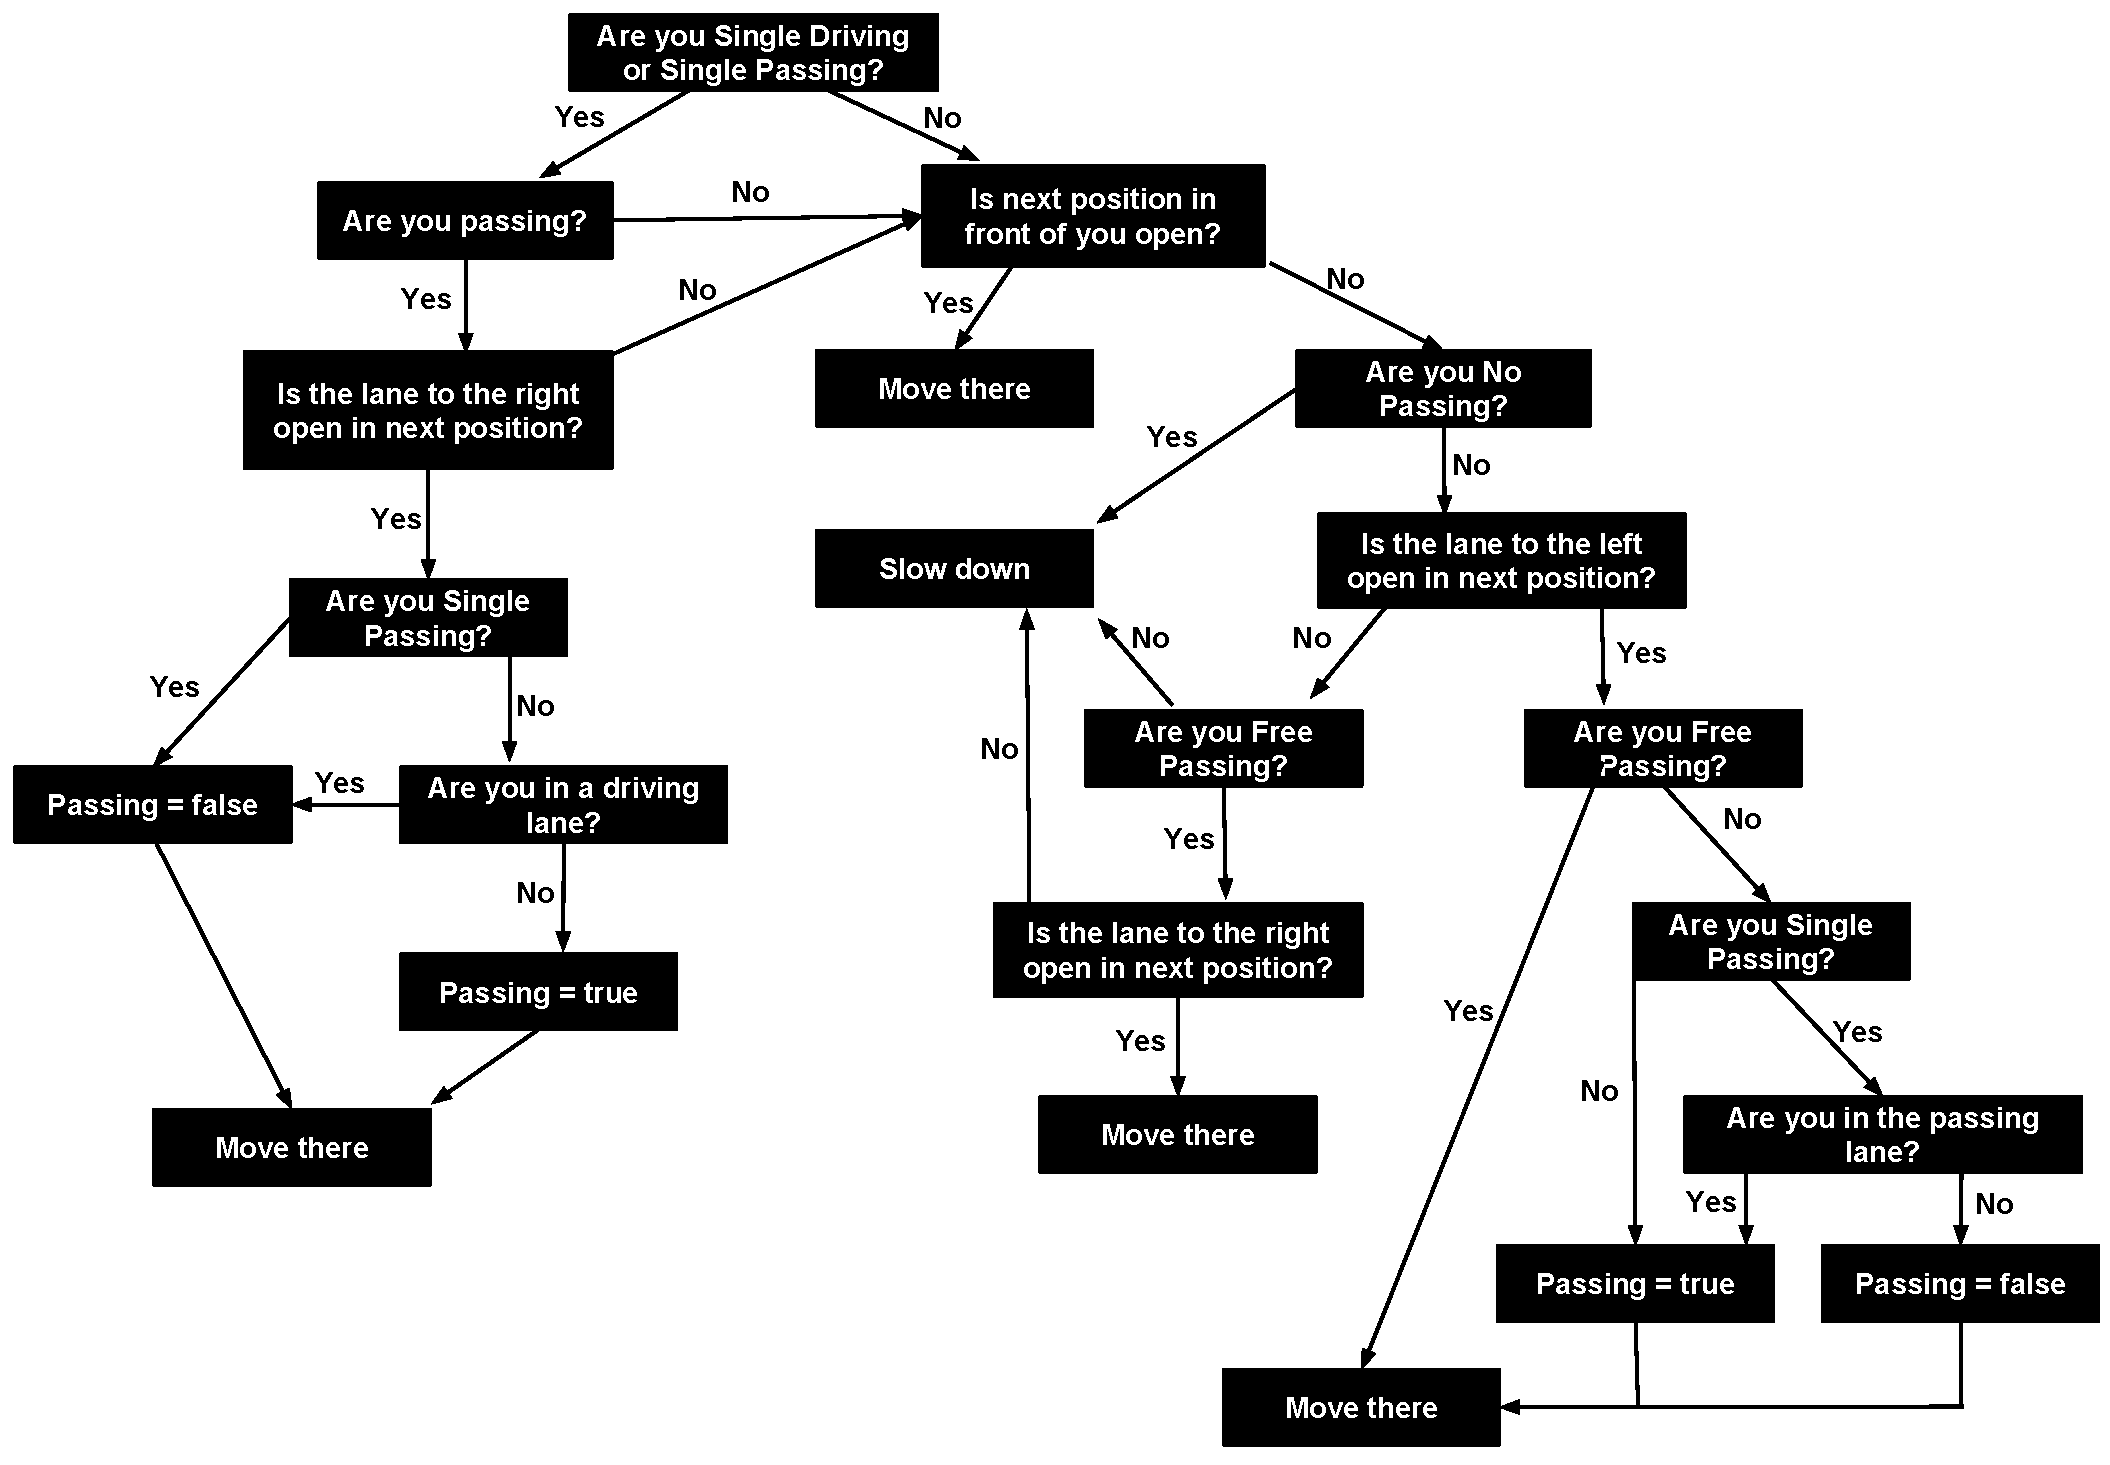
\includegraphics[scale=0.36]{MCM-LogicalFlowChartUpdated.pdf}
\caption{The Logic Flow Chart of the programming sequence.}
\label{MCM-LogicalFlowChart}	
\end{figure}

		\subsubsection{Program Execution Flow}		
			Now that we have discussed the overall class structure of our simulation program, we can explain the flow of execution of our simulation program. At the entry point of our simulation program, the user is prompted for the simulation parameters. Then, for each simulation specified by the number of simulations to run, our simulation program creates a new instance of the \texttt{Simulation} class and runs that simulation instance by calling the public instance method \texttt{Run()}. Next, within this public instance method (of the \texttt{Simulation} class), the collection of roads are generated and the cars are populated. The position of a vehicle is randomly generated using a uniform distribution, and the speed of a is randomized using our normal distribution model for possible vehicle speeds. After the roads have been populated with random cars, our simulation program begins looping through the number of iterations defined in the simulation parameters. Within each iteration, our simulation program 
\begin{figure}[h]
\centering
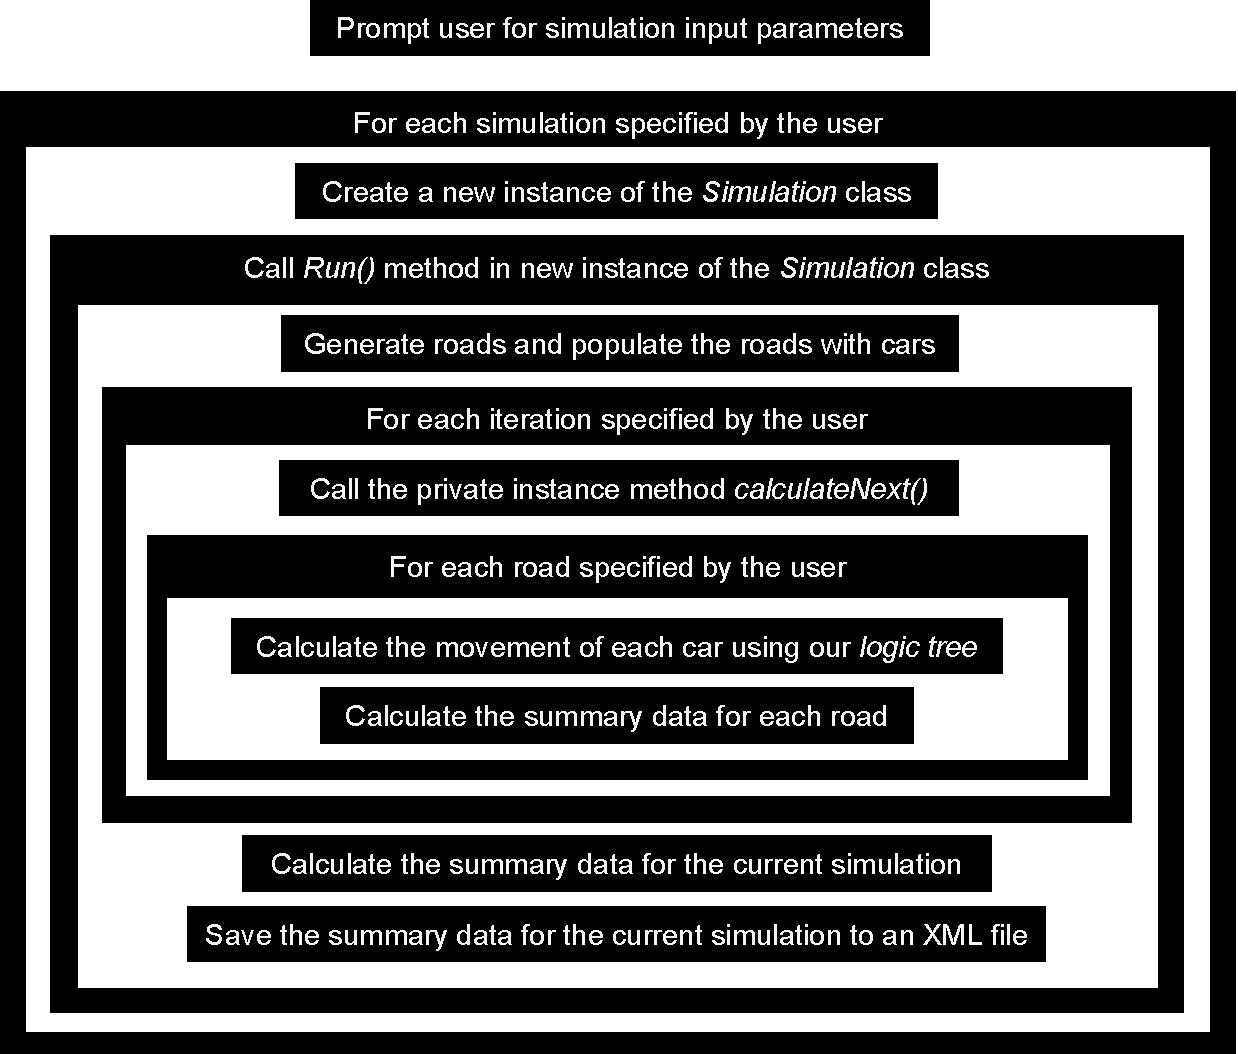
\includegraphics[scale=0.49]{MCMProgramFlow}
\caption{The Flow of Execution of the Simulation Program}
\label{MCMProgramFlow}
\end{figure}
implements our logic tree (see Figure ~\ref{MCM-LogicalFlowChart}.) to calculate new positions for each vehicle on each road. As soon as the execution of our logic tree finishes, our simulation program calculates the summary data for each road. Recall that each road in a simulation represents a different road type. After the simulation program finishes computing all the iterations specified by the simulation parameters, then the summary data for the whole simulation is calculated. At this point the simulation program is done computing iterations, so the simulation summary data is persisted in an XML file using an instance of the \texttt{DataPersistence} class. Finally, if there are multiple simulations defined by the simulation parameters, the simulation program iterates to the next simulation instance. (see Figure ~\ref{MCMProgramFlow}.)
			
		\subsubsection{Flaws and Improvements}
			Overall, the simulation program we developed implemented our model better than anticipated, especially within the time constraints. However, overall design flaws produced issues with the collection, persistence, and analysis of the simulation summary data. Initially, we attempted to collect and persist data for every vehicle on every road during every simulation. This method of collecting and persisting \emph{all} data would have required terabytes of storage space, which we did not have access to, nor time to analyze. So, we changed the way in which we collected and persisted data so that only the summary data for each iteration was stored in output XML file. However, we encountered several problems, mostly from time limitations, trying to import and analyze the data in Microsoft Excel. Thus, due to time constraints, we decided to only output summary data for each simulation. Therefore, when we continue to investigate this problem, we plan to use a database, instead of XML files, to persist our traffic data. A database would allow our simulation program to persist more information with an organizational structure that makes the statistical analysis of the data easier. Additionally, using a database to persist more data with better organization, would allow us to develop an extension of our simulation program that plays back the movement of traffic our simulation program calculated. This extension would allow us to analyze the traffic flow visually, instead of purely analytically. This would present us with the opportunity to catch further design flaws in both our model and implementation of the model.	
			

	
	\subsection{Probabilty Functions}
		\textit{Uniform distribution of vehicle position and lane}
			Our model utilized a standard random function found in the standard libraries for the OOPL(objected oriented programming language) we used to simulate our model. In initializing the lanes and slot for each individual vehicle in the model, the program used a uniform distribution to place the cars along the freeway in discrete positions for every rule and simulation considered. The purpose of this was to consider what a hot air balloon would actually see on a freeway from a fixed position and height when observed randomly. The affects of this assumption are considered later in the statistical summary of the data of our model. 

		\textit{Normal distribution of speeds} 
			To incorporate a more realistic simulation of what we intended to model, we designed a normal distribution to describe the initialization of every vehicle at the beginning of the simulation (See Figure ~\ref{MCMNormDist}.)
			
					
\begin{figure}[h]
\begin{center}
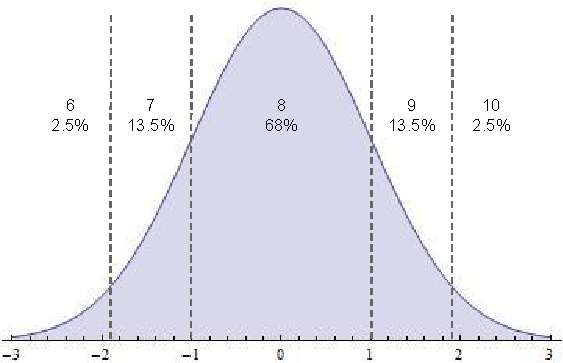
\includegraphics[scale=0.65]{MCM-speedsnormaldist}
\caption{Normal distribution graph of initial speed.}
\renewcommand{\figurename}{}
\label{MCMNormDist}
\end{center}
\end{figure}

		\textit{Probability of a Crash}
			In our model we only had two dynamics to allow for crashes due to interactions, namely from slowing down and from changing lanes. We initially intended to account for severity and probability of a crash to determine how traffic may be affected for any given rule and initial conditions but found that identifying an accurate probability for a crash due to slowing down or changing lanes proved more time consuming than originally thought and rejected the idea of considering severity. We also found difficulty in accounting for crash back ups in the coding and simulation of our model and determined it detracted from the actual test of which rule was better for light and heavy traffic. Our model then considered probability of an accident as merely a rating by which to determine the better rule based on certain output statistics of our simulation, particularly number of lane changes, number of times a vehicle slowed down, and number of times a vehicle failed a lane change due to our logic structure, i.e. there was a vehicle in its way when attempting to switch lanes(see logic structure). The formulation for the probability of  a crash had the following assumption and equations:\\
			\underline{\textit{Assumption}}
			\begin{itemize}
				\item The probability of slowing down and changing lanes are independent
				\item The probability of getting in an accident and changing lanes which we defined as a side-swipe accident was dependent
				\item The probability of getting in an accident and slowing down due to cars in front of you which we defined as a rear- end collision was dependent
			\end{itemize}
			\underline{\textit{Events}}
			\begin{itemize}
				\item A= The event there is an accident
				\item S = The event a vehicle has slowed down
				\item L = The event a vehicle has changed lanes
				\item D = The event the vehicle has to make a decision in the logic tree, i.e. slow down or change lane
			\end{itemize}
			\underline{\textit{Equations}}
			\begin{itemize}
				\item $P(A \cap S) = P(S)P(A|S)$ by the multiplication rule and dependence.
				\item $P(A \cap L) = P(L)P(A|L)$ by the multiplication rule and dependence.
				\item $P(S \cap L) = \emptyset$
				\item $P(A \cap D) = P\big(A \cap (S \cup L)\big)= P(A \cap L) + P(A \cap S)$ by deMorgan's law.
				\item $P(S) = \frac{X_S}{X_D}$
				\item $P(L) = \frac{X_L}{X_D}$
				\item $P(A|L)= .02$  by statistical data from the \cite{GovStats}.
				\item $P(A|S)= .204$ is to be determined by statistical data from the \cite{GovStats}.
			\end{itemize}
		
\section{\bfseries{Simulation Program Results}}

	Here is a tabular representation of the program's computational outputs:

\begin{figure}[h]
	\centering
	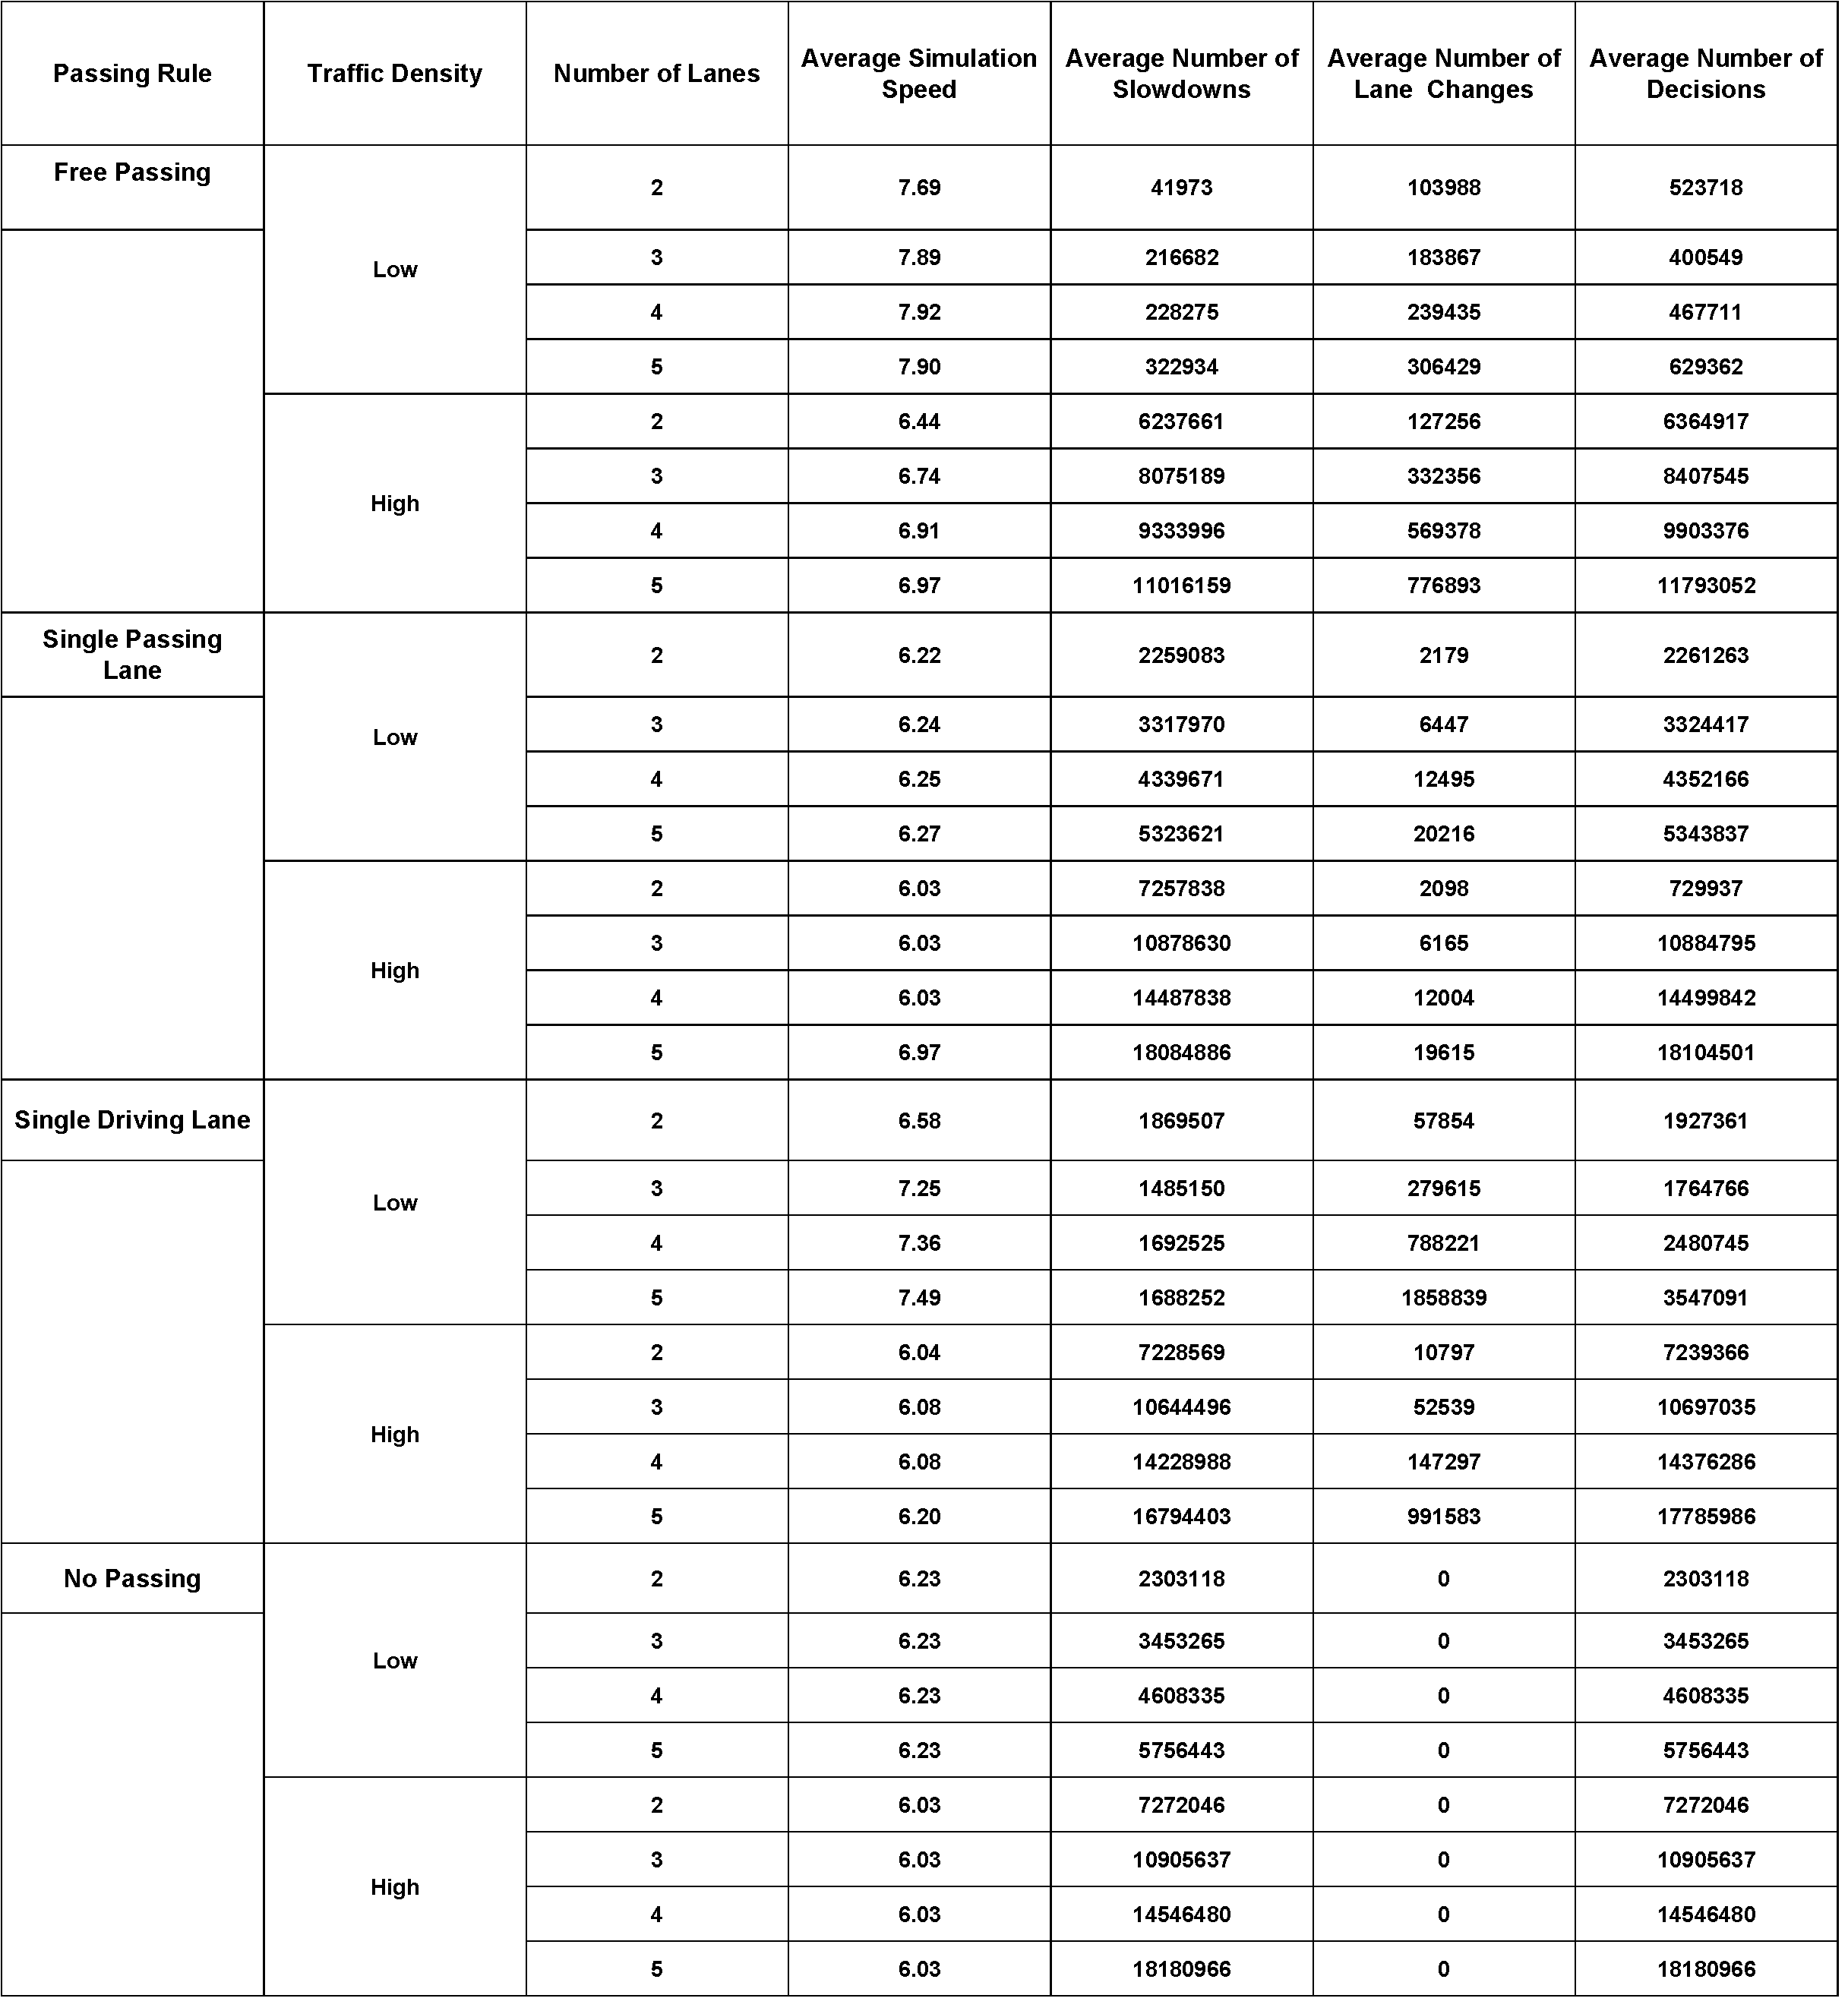
\includegraphics[scale=0.3]{MCMDataSummary}
	\caption{Computer program's computational outputs.}
	\label{MCMDataSummary}
	\end{figure}

\section{\bfseries{Statistical Analysis}}
	In our analysis of the data, to determine which rule is best, we consider three factors,namely the average flow, the average number of accidents, and the average speed for a given simulation with initial conditions:
	\begin{itemize}
		\item Density of cars ( High or low)
		\item Number of lanes(2,3,4,5)
	\end{itemize}
	
	\subsection{Definitions}
	
	\begin{itemize}
		\item \textit{Population}: Every possibly value for the output parameters of our simulation.
		\item \textit{Parameter}: A characteristic of the distribution of our Population, such as its mean and variance.
		\item \textit{Sample Statistics}: Point estimates of the parameters of a given Simulation.
		\item \textit{Sample}: One complete run of all iterations for a set of initial conditions for a simulation.
		\item \textit{Control Variables}: Parameters that stayed fixed for each road of the simulations, namely density and road length.
		\item \textit{Independent Variables}: The initial conditions used for each rode in a simulation.
		\item \textit{Dependent Variables}:  Output sample statistics of the model.
		\item\textit{Sample Size}: Number of simulations ran for a specific set of initial conditions.
		\item \textit{Significance level}: The probability of rejecting a test hypothesis, $H_0$, incorrectly( i.e. Stating there is enough statistical evidence to support the alternative hypothesis,$H_a$, when in truth the the null or test hypothesis was correct). 
	
	\end{itemize}

	\subsection{Assumptions}
	\begin{itemize}
		\item Each simulation is independent of previous simulations.
		\item The best point estimates of mean traffic flow and mean speed of a simulation(Sample) is the sum of these quantities respectively, for each iteration over the number of iterations in a simulation.
		\item The optimal rule to implement in traffic based on our model is determined by the highest average traffic flow, highest average speed, and lowest average accident rate of the samples.
		\item Control variables will not affect determination of best rule
		\item A sample size of 30 will be enough to statistically consider our data in terms of a z-statistic for hypothesis testing
		\item A $95\%$ confidence level will be significant enough to cover the true population parameter of interest.
	\end{itemize}
	
	
	\textit{Justifications}
	
		We can assume each simulation is independent because the initial conditions have a random probability distribution associated with their discrete values and every simulation has no prior knowledge of previous simulations.

		A Sample mean is the best unbiased estimate of the true value of a given population mean.
		
		Standard metrics of determining the implementation of particular highway policies are given be these sample statistics \cite{elvik2009handbook}.

		Many research papers use the simplifying assumption of conservation of cars, in order to find tractability in the model. Since this means that overall traffic density remains constant, we justify our assumption by considering the viewing space our model takes from a fixed position and fixed height over a highway during mid-day steady stream traffic \cite{seiboldconstructing}.
		By the central limit theorem, since we have the sample mean and variance and $n \geq 30$, we know we can approximate $W$ by $W=\frac{\bar x - \mu}{\sqrt{\frac{s^2}{n}}} \sim N(0,1)$.
		
		For reasonably centralized data $95\% $ significance is a strong test to use. The data being simulated by our model is only allowed to vary by some random independent variables and so the sample statistics are likely to show strong centralization. 	
		
	\subsection{Z-Statistic Hypothesis Test Analysis}
	From our results we noticed that for nearly all road types the rule with the highest average of traffic flow, average simulation speed, and lowest safety rating was the free passing rule, while many of the other rules showed insignificant difference in simulation summary figures. However, one rule did standout from our results as a potential candidate to make a comparison with, the single driving lane. We tested the hypothesis that the free passing was indeed the best rule to implement based on our results. The single driving lane rule performed unremarkably in the low number of lanes simulations, but as lanes increased this rule seemed to demonstrate improvement in all three categories in consideration. Thus, we only performed hypothesis testing on these two rules. Our sample size was n = 30, which represented number of simulations whose summary data we averaged over all the samples. When testings the difference of two sample means, as long as the criterion that $n \geq 30$ is met, we can  reasonably approximate the sampling distribution as a Normal model with mean 0 and standard deviation 1. Hence, for the sample statistics $\bar q$ and $\bar v$ we can prove whether free passing is truly the best rule for all cases. For reference, the one-tailed hypothesis test and test statistic we used was the difference of means z- statistic with large sample size($n\geq30$) \cite{FundTrafficEng}: 	
	\begin{align*}
		H_o : &\mu_1 - \mu_2 \leq 0\\
		H_a : &\mu_1 - \mu_2 >0\\
		z_0 = &\frac{(\bar x_1 - \bar x_2) - (\mu_1 - \mu_2)}{\sqrt{\frac{1}{n}(s_1^2 + s_2^2)}}
	\end{align*}
	
	The $95\%$ confidence level determines the rejection region we will use, in particular we will reject the null hypothesis for test values of z which are greater than 1.645, formally:
	\begin{align*}
		R.R. = \{ z | z>1.645\}
	\end{align*}
\begin{figure}[h]
	\centering
	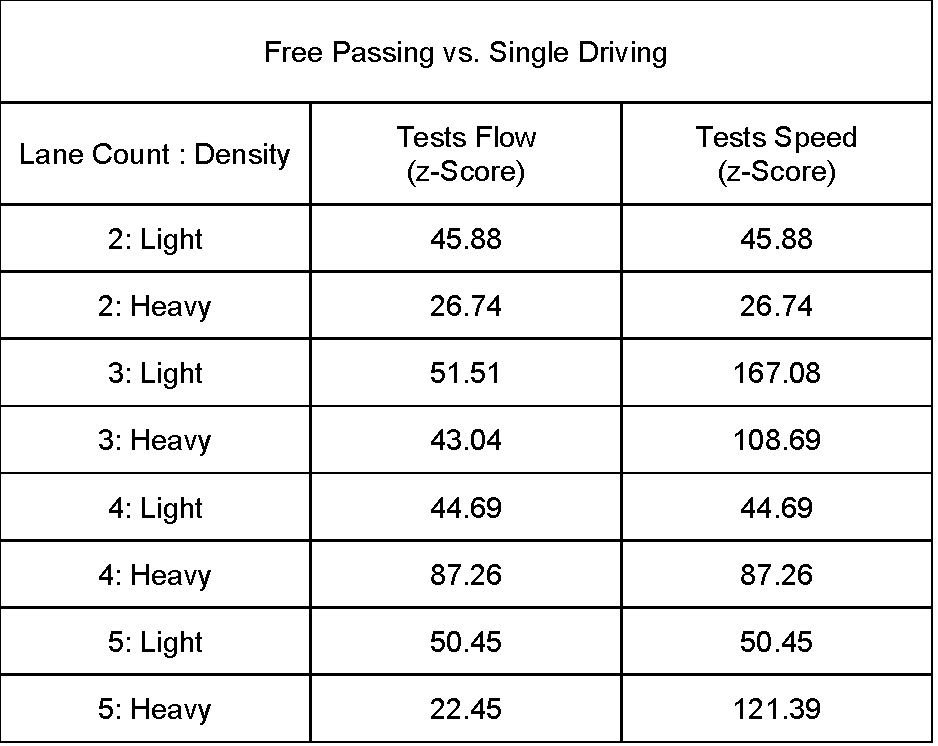
\includegraphics[scale=0.4]{MCMProbablityZ}
	\caption{One Tailed Difference of Means Z-Statistic Hypothesis Test}
	\label{MCMProbabilityZ}
	\end{figure}
	
	\subsection{Statistical Summary}A table of our sample statistics is provided below:
	
	\begin{figure}[h]
	\centering
	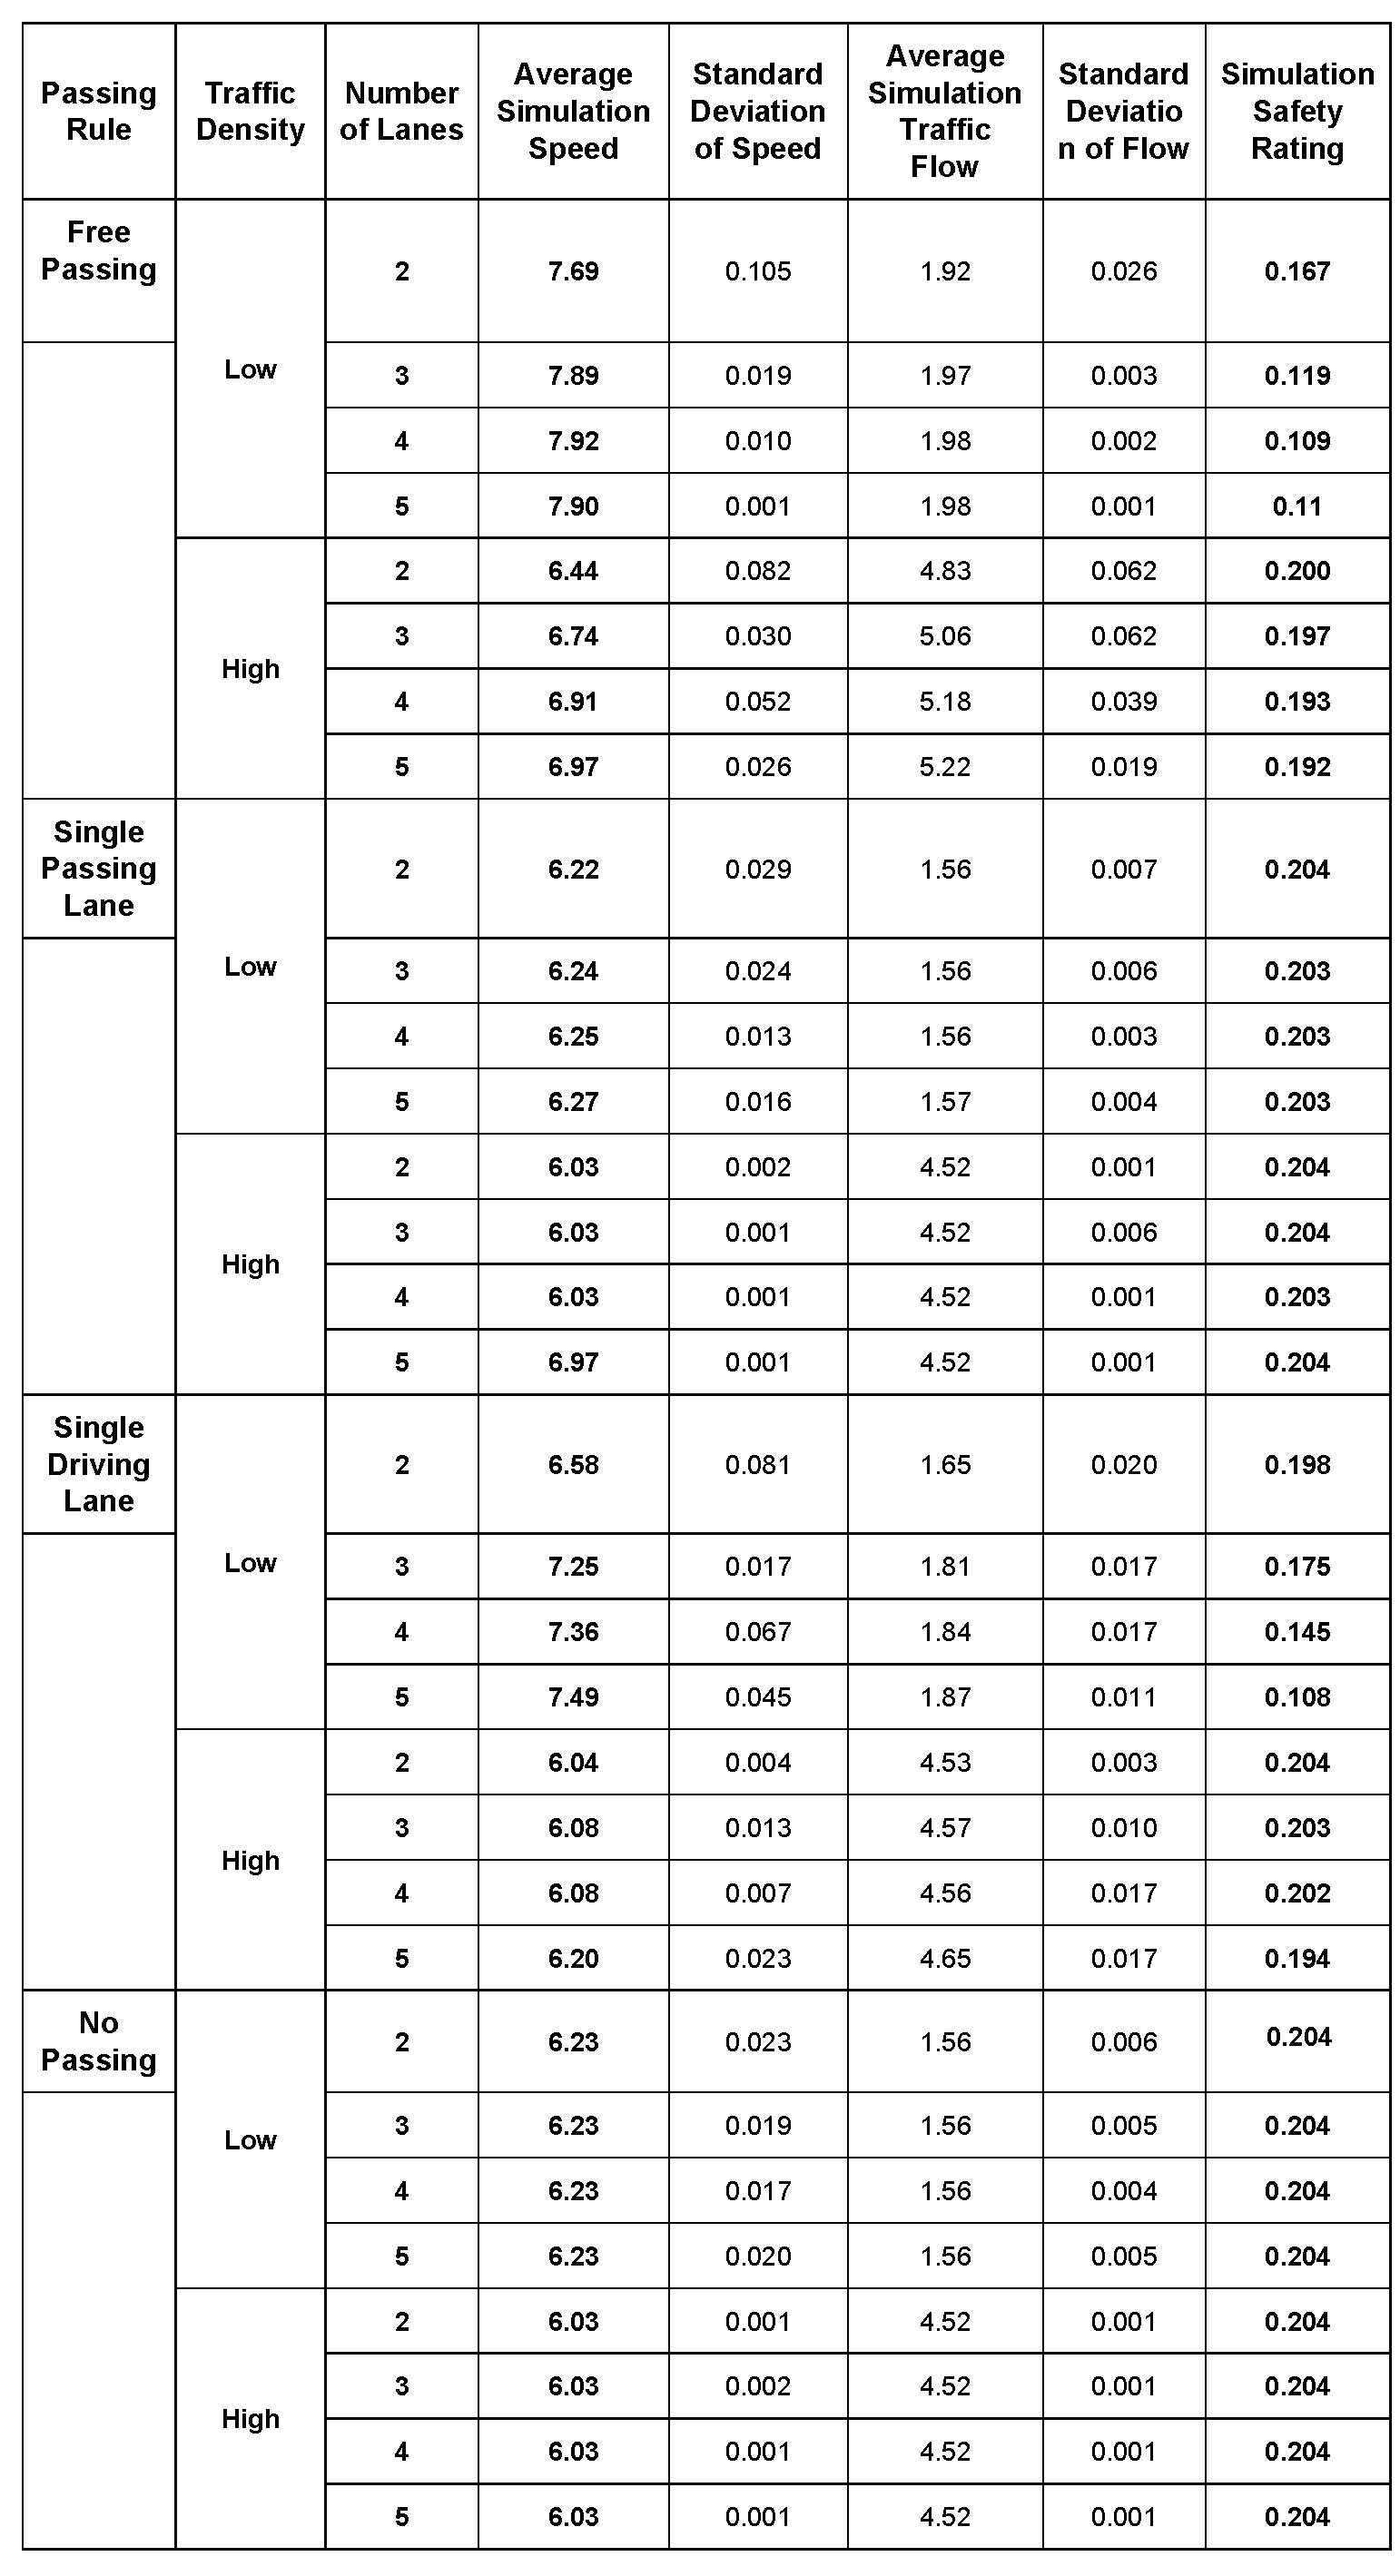
\includegraphics[scale=0.25]{MCMStatisticalAnalysisOfTrafficFlow}
	\caption{Calculated Statistical Data}
	\label{MCMStatisticalAnalysisOfTrafficFlow}
	\end{figure}
	

	From our analysis we determine in the simulations of lanes 1 through 4 with low density and 1 through 5 with high density, the sample statistics for the free passing rule was significantly better then the rest. In fact, performing a p-value test on just one case, that is, measuring the probability of finding a more extreme value than z, we find 
	\[
		P( z > z_0) = 6.83 \e{-460}.
	\]
	This is a clear indication there is a flaw in our model because values this extreme are not only incredibly unlikely but too significant to consider as credible evidence. We believe the error could be contained in how the statistics are drawn from each simulation or how the program steps through its logic decision loop. Because of this we determine our hypothesis testing of the sample means $\bar q$ and $\bar v$ are inconclusive. This may be due to a variety of influential factors,but we believe there is a very strong likelihood that these results stem from the minuscule standard deviations of the sample statistics. However, these were not the only characteristics in determining an optimal rule, we are still left with the simulation safety rating of each rule. From our statistical analysis summary above we see that free passing still was the dominant rule in terms of most safe, i.e. smallest safety rating, nevertheless the single driving still persists and proves to be the safest rule when the simulation has 5 lanes and low density. 

	\subsection{Statistical Analysis Difficulties}
	The data formatting was the most difficult part in the statistical analysis. At first we attempted to analyze the data on a iterations basis for each simulation by summing over the average iteration speed and dividing by 500, the total number of iterations. However in the XML(Extensible Markup Language) format that we used for persisting data, calculating the average of these iteration velocities for every simulation proved to be too difficult and time consuming in excel without using some type of XML to excel macro, which we were unskilled in. We did however achieve to find the sample statistics of average safety factor, average simulation velocity, and average traffic flow for a single road type, the 2 lane low density initial conditions. To overcome this unforeseen difficulty, we went back to the model in our object-oriented programming language and performed the simulation summaries which calculated the sample statistics for each simulation at the simulation summary data type level rather than the iteration summary level, which minimized the time to determine the averages over all our samples that was used for our statistical analysis.

\section{\bfseries{Strengths and Weaknesses}}

	\subsection{Strengths}
		Our model took a unique approach to a problem which few other researches have truly considered. The modeling of a particle model for dynamics of a macro system is extremely difficult in finding tractable assumptions to make realistic solutions. The strengths of our model is that we attempted to put each of its elements into practical and concrete situations that explains its place in real life and  provide a frame work to build other concept on top of. The amount of data about the model from the simulation can provide insights into a multitude of other questions which we have full intent to investigating. Another strength in the assumptions we made is that a simple switch of orientation would provide exactly the same outcome so further simulation is not needed, our logic based decision tree is non-oriented and so allows for direction to be changed regardless of rules implemented.
		
	\subsection{Weaknesses}
		A major set back of our model was its inability to accurately and definitively provide conclusive proof that a particular rule was better than all others within reason. This drawback did not prevent our ability to draw other conclusions from the model and indeed we now know what types of considerations must be taken, namely direct observation of parameters should always be preferred over averages of summary information. Furthermore, our limited time prevented us from implementing a mixed rule model which ideally would represent freedom of judge for a given simulation and parameters. Information about how such a system would behave can still be drawn from behavior of our current system, however our model's strict adherence to a specific rule seems more representative of an intelligently controlled traffic system.
		 
\section{\bfseries{Conclusion}}
	In conclusion, we believe our simulation was successful in modeling traffic dynamics in order to answer the question of how the stay-right-rule except to pass in light and heavy traffic. Many of the assumptions made were independently verified by external sources and proved to show effective dynamics in varying conditions. We found that there was limited trade off between traffic flow and safety and in fact, it was often the systems with the best traffic flow were the safest as well. We infer this is because freeways which are more congested, i.e slower traffic flow, have a higher probability of an interaction which results in an accident irrelevant of traffic density. Hence based on our model, we conclude that traffic flow and the probability of getting in an accident are inversely proportional to the extent that the average speed of the system does not approach grid lock. Furthermore, we found that number of traffic lanes plays a unique role in the traffic dynamics of each rule and whether it was effective in various traffic densities. In particular, the stay-right-rule which we defined as the single driving lane rule became more effective in terms of average speed, average flow rate, and safety factor as the number of lanes increased. We deduce this is due to the mechanics of the logic system it follows in which, the rule prefers open spaces in order to best cascade around cars and then collapse back to a single lane. We further predict that as we watch this segment of cars go indefinitely, due to the looping from the conservation of cars assumption we believe formation of packs should begin to emerge and will eventually reach complete segregation by the time our iterations of watching reaches infinity. Our final words are that traffic dynamics are challenging and intriguing. We have learned that often in modeling a situation, it is helpful to make assumptions of systems that are already known and simplify their models in order to match the problem you wish to consider, however other times it is best to originate a completely new idea and test its outcomes against known models that exists. 

\section{\bfseries{Future Work}}
	With the development of our program there are opportunities to adjust the starting conditions and individual vehicle interactions. Therefore the programs parameters can be changed in order to make the model more practical to the real world or to test different traffic flow questions. With this ability in our model some variations should be tested but could not be completed within the time frame. 
	\subsection{Individualized Vehicle Rules}
	In our model we defined road rules where everyone on a highway followed the same set of passing rules. This was a simplification assumptions in order to increase both programming and analysis time. The problem here is that slow cars have the ability to start in the fast lanes and can get stuck there for a prolonged time. Situations as slow cars in fast lanes does happen in real situations but not in the large scale that our model allows it. 
	The big variation that would be further followed would be to assign individual vehicles a passing rule instead of everyone on the same highway a passing rule. This highly increases the realism of our model since every driver has their own average speed they tend to travel. Furthermore, this implication would help diminish the intelligent design factor that has overrun our program. In our current model everyone follows the rule no matter the interaction. This insistence to follow the passing rule would be still upheld in the individualized vehicle passing rules but by varying what type of rules are seen on a highway we can model a more realistic road. 
	
	\subsection{Variations in Driver Psychology}
	One model we found attempted to test individual driver psychology. This acts as a subdivision of the varying speed adjustment. Driver's may be influenced by perceived safety, age, likelihood to be distracted, emotional distress, etc. Furthermore in this study of the psychology of individual drivers there is the consideration that drivers can only perceive things in a limited viewing frame and, thus, only varying their speed to match the vehicles around them ~\cite{burghout2005}. These are attributes that can easily be implemented into our program and would be interesting to pursue. By using a small set of simple assumptions our program could begin to describe some of these variations by changing the logic tree system which governs interactions in the simulation.  

\newpage
\section{\bfseries{References}}
\bibliography{References}

\end{document}
